\documentclass[11pt,a4paper]{article}

% Packages
\usepackage[utf8]{inputenc}
\usepackage[T1]{fontenc}
\usepackage{amsmath,amssymb}
\usepackage{mathptmx}
\usepackage[margin=1in]{geometry}
\usepackage{graphicx}
\usepackage{booktabs}
\usepackage{array}
\usepackage{hyperref}
\usepackage{xcolor}
\usepackage{float}
\usepackage{caption}
\usepackage{subcaption}
\usepackage{natbib}
\usepackage{fancybox}
\usepackage{setspace}

\hypersetup{
    colorlinks=true,
    linkcolor=blue,
    citecolor=blue,
    urlcolor=cyan,
    pdftitle={Stochastic Incompleteness in LLM Summarization: A Predictability Taxonomy for Clinical AI Deployment},
    pdfauthor={Laxman M M},
}

\title{\LARGE\textbf{Stochastic Incompleteness in LLM Summarization:\\A Predictability Taxonomy for Clinical AI Deployment}}

\author{
    \textbf{Dr.\ Laxman M M, MBBS}\\
    Government Duty Medical Officer, PHC Manchi\\
    Bantwal Taluk, Dakshina Kannada, Karnataka, India\\
    DNB General Medicine Resident (2026), KC General Hospital, Bangalore\\
    Email: \texttt{barlax5377@gmail.com}\\
    ORCID: \href{https://orcid.org/0009-0009-0405-6531}{0009-0009-0405-6531}
}

\date{February 2026}

\begin{document}

\maketitle

\begin{center}
\fbox{\parbox{0.9\textwidth}{
\textbf{Paper 5 of the MCH Research Program} --- This paper extends the variance analysis framework from Paper~4 into a practical deployment taxonomy. We demonstrate that accuracy and output predictability are independent dimensions for clinical AI assessment, yielding a four-class behavioral taxonomy (IDEAL, EMPTY, DIVERGENT, RICH) and identifying stochastic incompleteness as a novel failure mode invisible to standard benchmarks.
}}
\end{center}

\vspace{0.5em}

% ============================================
% ABSTRACT
% ============================================
\begin{abstract}
\noindent Standard accuracy benchmarks evaluate whether a language model produces correct outputs but not whether it produces them consistently. We demonstrate that accuracy and output predictability are independent dimensions by analyzing 8 medical LLMs at a clinical summarization position (P30, STEMI case history). Cross-model accuracy verification against a 16-element clinical rubric reveals no significant correlation between Variance Ratio ($\text{Var\_Ratio} = \text{Var}_{\text{TRUE}} / \text{Var}_{\text{COLD}}$) and task accuracy (Pearson $r = -0.24$, $p = 0.56$, $N = 8$). This independence yields a four-class behavioral taxonomy: \textbf{IDEAL} (convergent, accurate; 4 models), \textbf{EMPTY} (convergent, inaccurate; Gemini Flash, 16\% accuracy despite low variance), \textbf{DIVERGENT} (high variance, incomplete; Llama 4 Scout $\text{Var\_Ratio} = 7.46$, Llama 4 Maverick $\text{Var\_Ratio} = 2.64$), and \textbf{RICH} (moderate variance, highly accurate; Qwen3 235B, 95\% accuracy). The DIVERGENT class exhibits a novel failure mode---stochastic incompleteness---in which summaries are factually accurate but randomly incomplete: identical prompts produce summaries covering 5/16 to 14/16 clinical elements across trials, with zero hallucinations. This failure mode is invisible to standard benchmarks. The EMPTY class demonstrates a complementary blind spot: convergent outputs that lack clinical content. We propose a two-dimensional deployment framework ($\text{Var\_Ratio} \times \text{Accuracy}$) as a minimum requirement for clinical AI assessment.

\vspace{0.5em}
\noindent\textbf{Keywords:} clinical AI deployment, predictability taxonomy, stochastic incompleteness, variance ratio, hallucination detection, medical summarization, LLM safety
\end{abstract}

% ============================================
% 1. INTRODUCTION
% ============================================
\section{Introduction}

The deployment of language models in clinical settings requires that outputs be both accurate and predictable. A model that produces correct summaries on average but varies wildly across trials poses a risk: any individual output may omit critical information, with no indication that information is missing.

Prior work in the MCH Research Program established that context sensitivity ($\Delta$RCI) varies across architectures \citep{laxman2026paper1,laxman2026paper2}, follows task-specific temporal patterns \citep{laxman2026paper3}, and can be characterized through variance analysis \citep{laxman2026paper4}. Paper~4 identified an anomaly: two Llama models showed extreme output variance ($\text{Var\_Ratio}$ up to 7.46) at the medical summarization position, suggesting a potential safety concern.

This paper extends that observation into a systematic framework. We ask: does output variance predict task accuracy? If not, what is the structure of the $\text{Var\_Ratio}$--accuracy relationship?

We find that the relationship is categorical, not continuous. $\text{Var\_Ratio}$ and accuracy are statistically independent ($r = -0.24$, $p = 0.56$), and four distinct behavioral classes emerge. Each class represents a different failure mode or success pattern that is invisible when only one dimension is assessed. In particular, we identify \textbf{stochastic incompleteness}---a failure mode in which outputs are factually sound but randomly incomplete---as a clinically relevant risk that standard accuracy benchmarks do not detect.

% ============================================
% 2. METHODS
% ============================================
\section{Methods}

\subsection{Experimental Design}

We analyzed 8 medical LLMs at position 30 (P30) of a 29-exchange STEMI case history. P30 used a summarization prompt (``Summarize this case...'') that requires integration of accumulated clinical information. Each model was evaluated for 50 independent trials under identical conditions: temperature = 0.7, max\_tokens = 1024, embedding model = all-MiniLM-L6-v2 (384-dimensional) \citep{reimers2019sentence}.

This analysis uses the 8-model medical subset from Paper~2's 14-model dataset (112,500 total responses across 25 model-domain runs). Only models with complete response text preserved at P30 are included, as accuracy scoring requires access to raw summaries.

\subsection{Models}

\begin{table}[H]
\centering
\begin{tabular}{llll}
\toprule
\textbf{Model} & \textbf{Vendor} & \textbf{Architecture} & \textbf{Parameters} \\
\midrule
DeepSeek V3.1 & DeepSeek & Dense/MoE & 671B (37B active) \\
Gemini Flash & Google & Undisclosed & Undisclosed \\
Ministral 14B & Mistral & Dense & 14B \\
Kimi K2 & Moonshot & MoE & $\sim$1T (32B active) \\
Mistral Small 24B & Mistral & Dense & 24B \\
Qwen3 235B & Alibaba & MoE & 235B (22B active) \\
Llama 4 Maverick & Meta & MoE & 400B (17B active) \\
Llama 4 Scout & Meta & MoE & 109B (17B active) \\
\bottomrule
\end{tabular}
\caption{Model set. All 8 models are from the medical domain subset of Paper~2's 14-model benchmark ($N = 360$ position-level measurements from 12 model-domain runs in Paper~4).}
\label{tab:models}
\end{table}

\subsection{Accuracy Rubric}

We developed a 16-element clinical rubric spanning the full STEMI case trajectory:

\begin{table}[H]
\centering
\begin{tabular}{ll}
\toprule
\textbf{Phase} & \textbf{Elements} \\
\midrule
Presentation (P1--P5) & STEMI diagnosis, age 52 male, chest pain \\
Diagnostics (P6--P10) & Troponin elevated, ECG ST-elevation, LAD occlusion, EF 45\% \\
Intervention (P11--P15) & PCI performed, RV involvement, hypotension management \\
Complications (P16--P20) & New murmur, mitral regurgitation (day 2) \\
Recovery (P21--P29) & Secondary prevention, cardiac rehab, lifestyle modification, \\
                     & return to work, follow-up \\
\bottomrule
\end{tabular}
\caption{16-element clinical rubric for STEMI case summarization. Each element was scored as present (1) or absent (0) using regex pattern matching against response text.}
\label{tab:rubric}
\end{table}

Each element was scored as present (1) or absent (0) using regex pattern matching against the response text. Accuracy = (elements present) / 16. All 50 TRUE-condition P30 responses were scored per model.

\subsection{Variance Ratio}

$\text{Var\_Ratio}$ at P30 was computed from embedding-level analysis (Paper~4):
\begin{equation}
\text{Var\_Ratio} = \frac{\text{Var}(\text{TRUE embeddings})}{\text{Var}(\text{COLD embeddings})}
\end{equation}
across 50 trials, where variance is the mean variance across all 384 embedding dimensions. Values are position-specific (P30 only) rather than model-level averages.

\subsection{Statistical Analysis}

The primary test is the Pearson correlation between $\text{Var\_Ratio}$ and mean accuracy (\%) across 8 models. We also computed Spearman rank correlation and tested quadratic models to assess whether the relationship is continuous, monotonic, or categorical.

% ============================================
% 3. RESULTS
% ============================================
\section{Results}

\subsection{Cross-model accuracy}

\begin{table}[H]
\centering
\begin{tabular}{lcccccc}
\toprule
\textbf{Model} & \textbf{Var\_Ratio} & \textbf{Mean Acc (\%)} & \textbf{Std} & \textbf{Range} & \textbf{Perfect (16/16)} & \textbf{Class} \\
\midrule
DeepSeek V3.1 & 0.48 & 82.8 & 1.23 & 10--16 & 2/50 & IDEAL \\
Gemini Flash & 0.60 & 15.8 & 2.88 & 0--16 & 1/50 & EMPTY \\
Ministral 14B & 0.75 & 90.2 & 1.71 & 7--16 & 10/50 & IDEAL \\
Kimi K2 & 0.97 & 91.9 & 1.04 & 11--16 & 13/50 & IDEAL \\
Mistral Small 24B & 1.02 & 82.6 & 1.25 & 10--16 & 1/50 & IDEAL \\
Qwen3 235B & 1.45 & 95.2 & 0.86 & 13--16 & 23/50 & RICH \\
Llama 4 Maverick & 2.64 & 46.8 & 1.33 & 5--11 & 0/50 & DIVERGENT \\
Llama 4 Scout & 7.46 & 55.4 & 1.78 & 5--14 & 0/50 & DIVERGENT \\
\bottomrule
\end{tabular}
\caption{Cross-model P30 medical accuracy and variance. Class assignments based on $\text{Var\_Ratio} \times \text{Accuracy}$ quadrant analysis.}
\label{tab:accuracy}
\end{table}

\subsection{Accuracy and Var\_Ratio are independent}

\begin{table}[H]
\centering
\begin{tabular}{lccc}
\toprule
\textbf{Metric pair} & \textbf{Pearson $r$} & \textbf{$p$-value} & \textbf{Spearman $\rho$} \\
\midrule
$\text{Var\_Ratio}$ vs Accuracy & $-0.24$ & 0.56 & $-0.07$ \\
\bottomrule
\end{tabular}
\caption{Correlation analysis. No significant linear or monotonic correlation exists between $\text{Var\_Ratio}$ and accuracy ($p = 0.56$, Spearman $p = 0.87$). The relationship is categorical, not continuous.}
\label{tab:correlation}
\end{table}

No significant linear or monotonic correlation exists between $\text{Var\_Ratio}$ and accuracy. A quadratic model (testing for a U-shaped or inverted-U relationship) also failed to reach significance ($R^2 = 0.11$, F-test $p = 0.72$). The relationship between $\text{Var\_Ratio}$ and task performance is \textbf{categorical, not continuous}: models cluster into distinct behavioral classes rather than following a smooth function.

\begin{figure}[H]
    \centering
    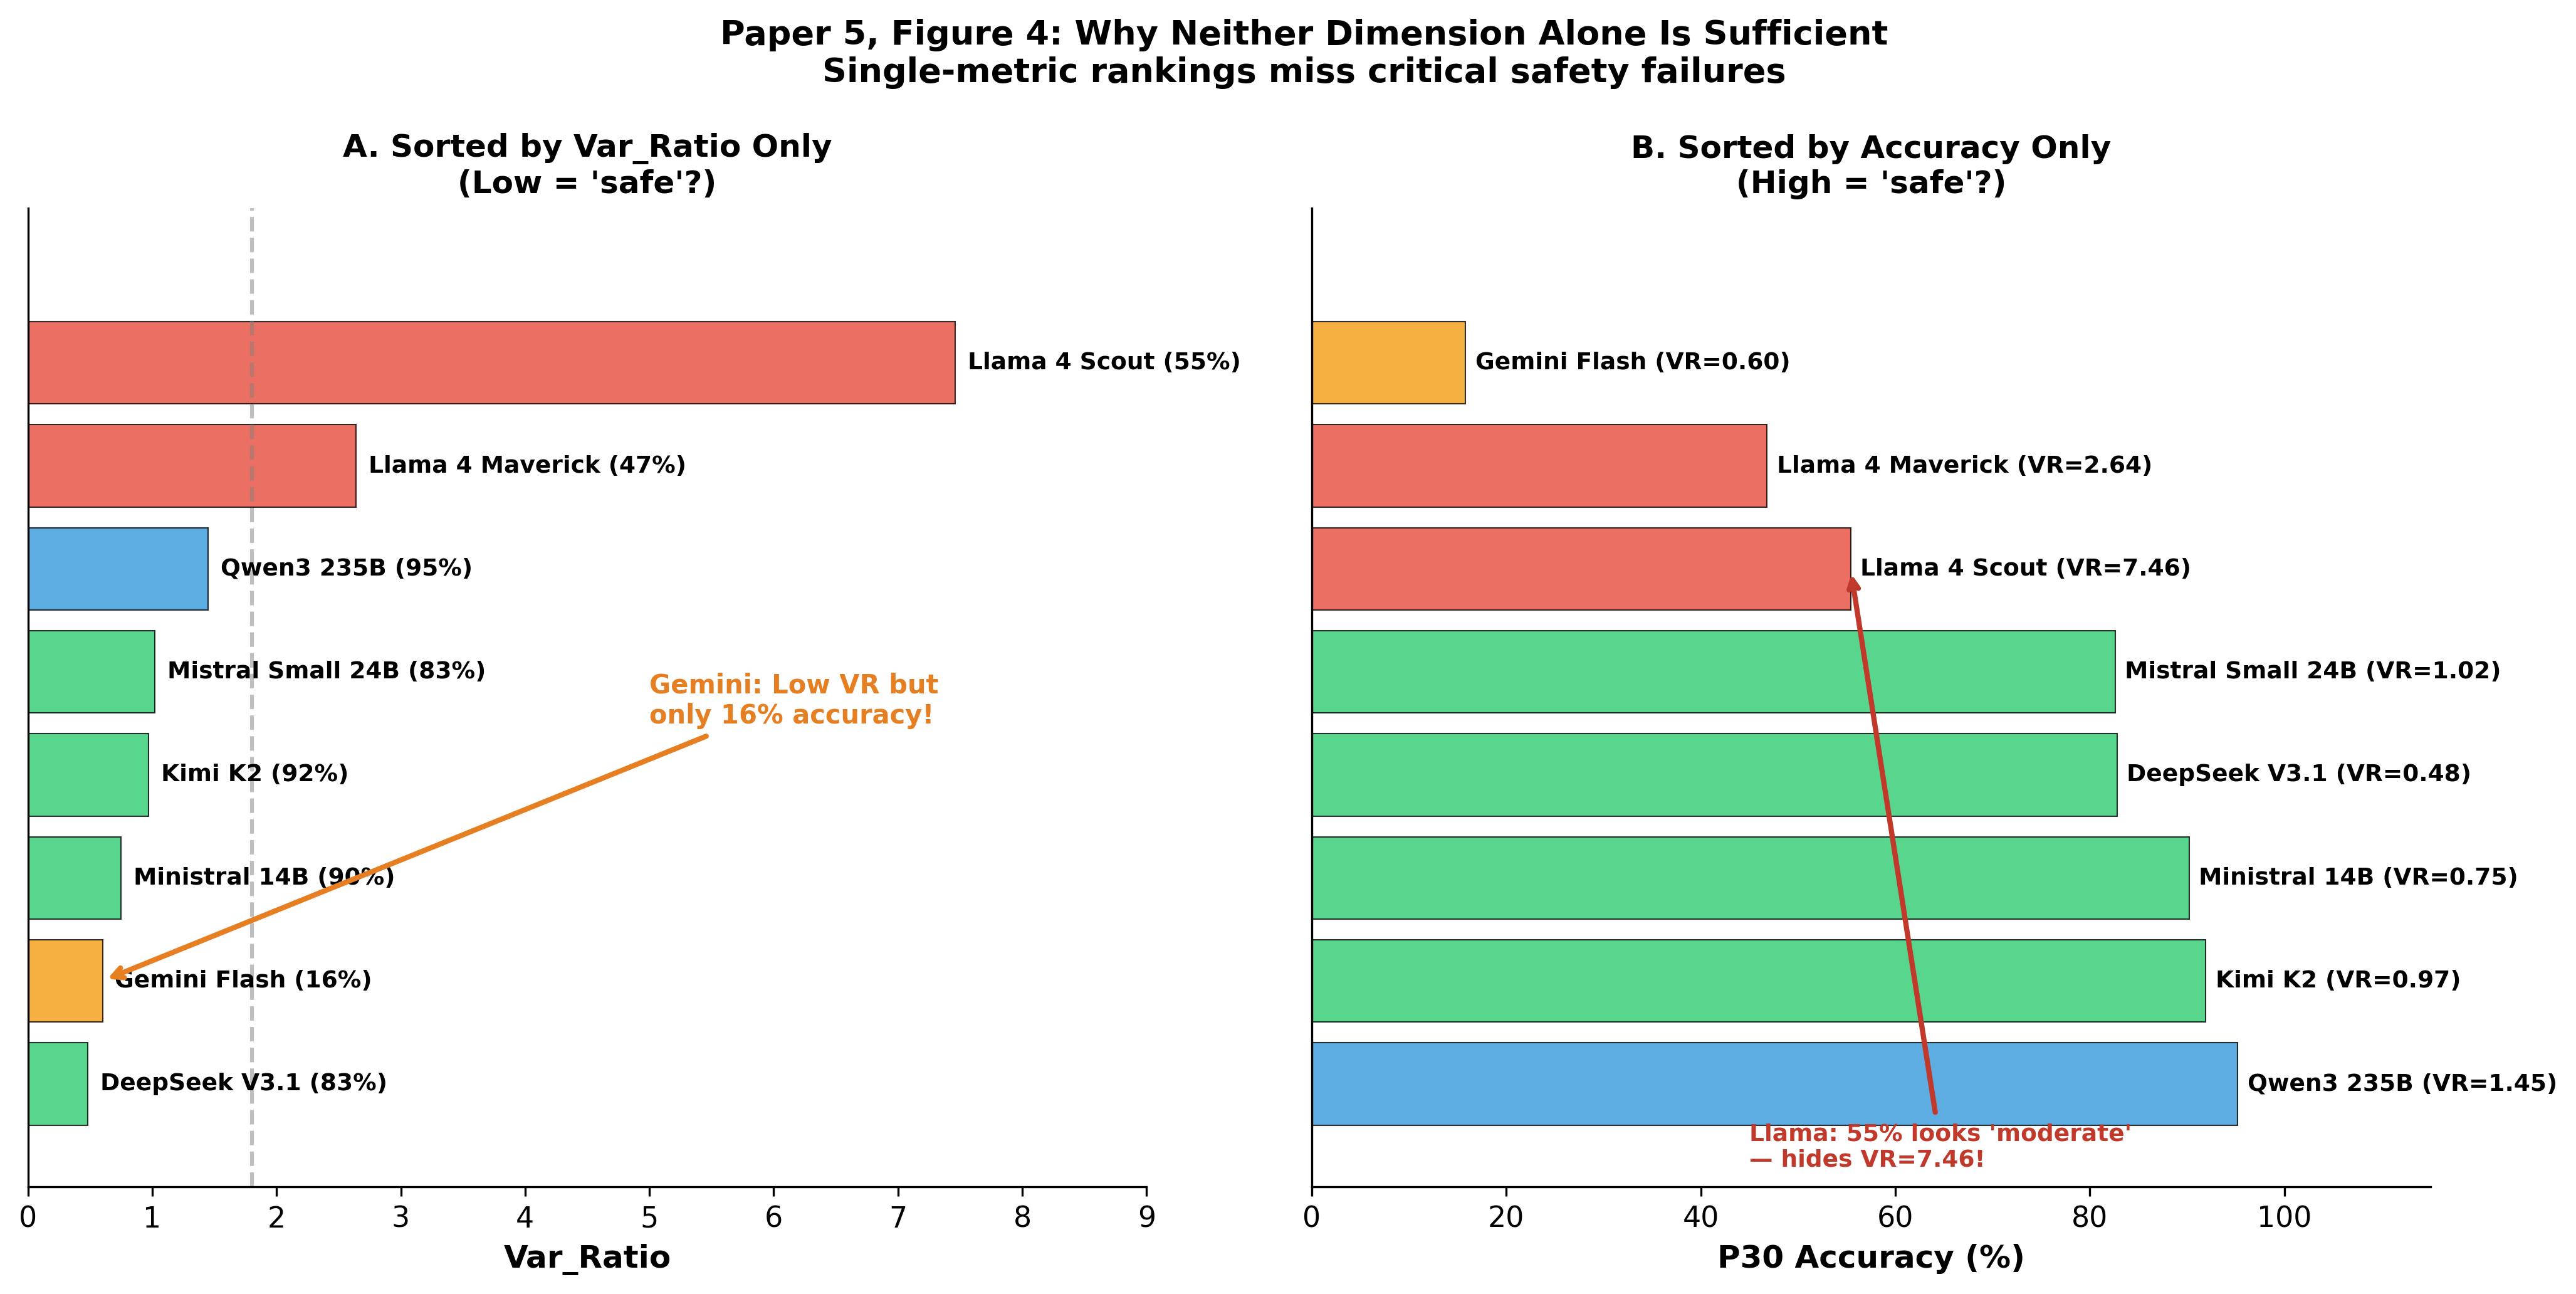
\includegraphics[width=0.95\textwidth]{../figures/fig4_one_dimension_failure.png}
    \caption{\textbf{Why neither dimension alone is sufficient.} Left: $\text{Var\_Ratio}$ alone cannot distinguish IDEAL from EMPTY (both low variance, but Gemini Flash has 16\% accuracy). Right: Accuracy alone cannot distinguish IDEAL from DIVERGENT at the individual-trial level (a single Llama trial may score adequately, but the next may not).}
    \label{fig:one_dimension}
\end{figure}

\subsection{Four-class predictability taxonomy}

The independence of $\text{Var\_Ratio}$ and accuracy yields a $2 \times 2$ taxonomy:

\begin{figure}[H]
    \centering
    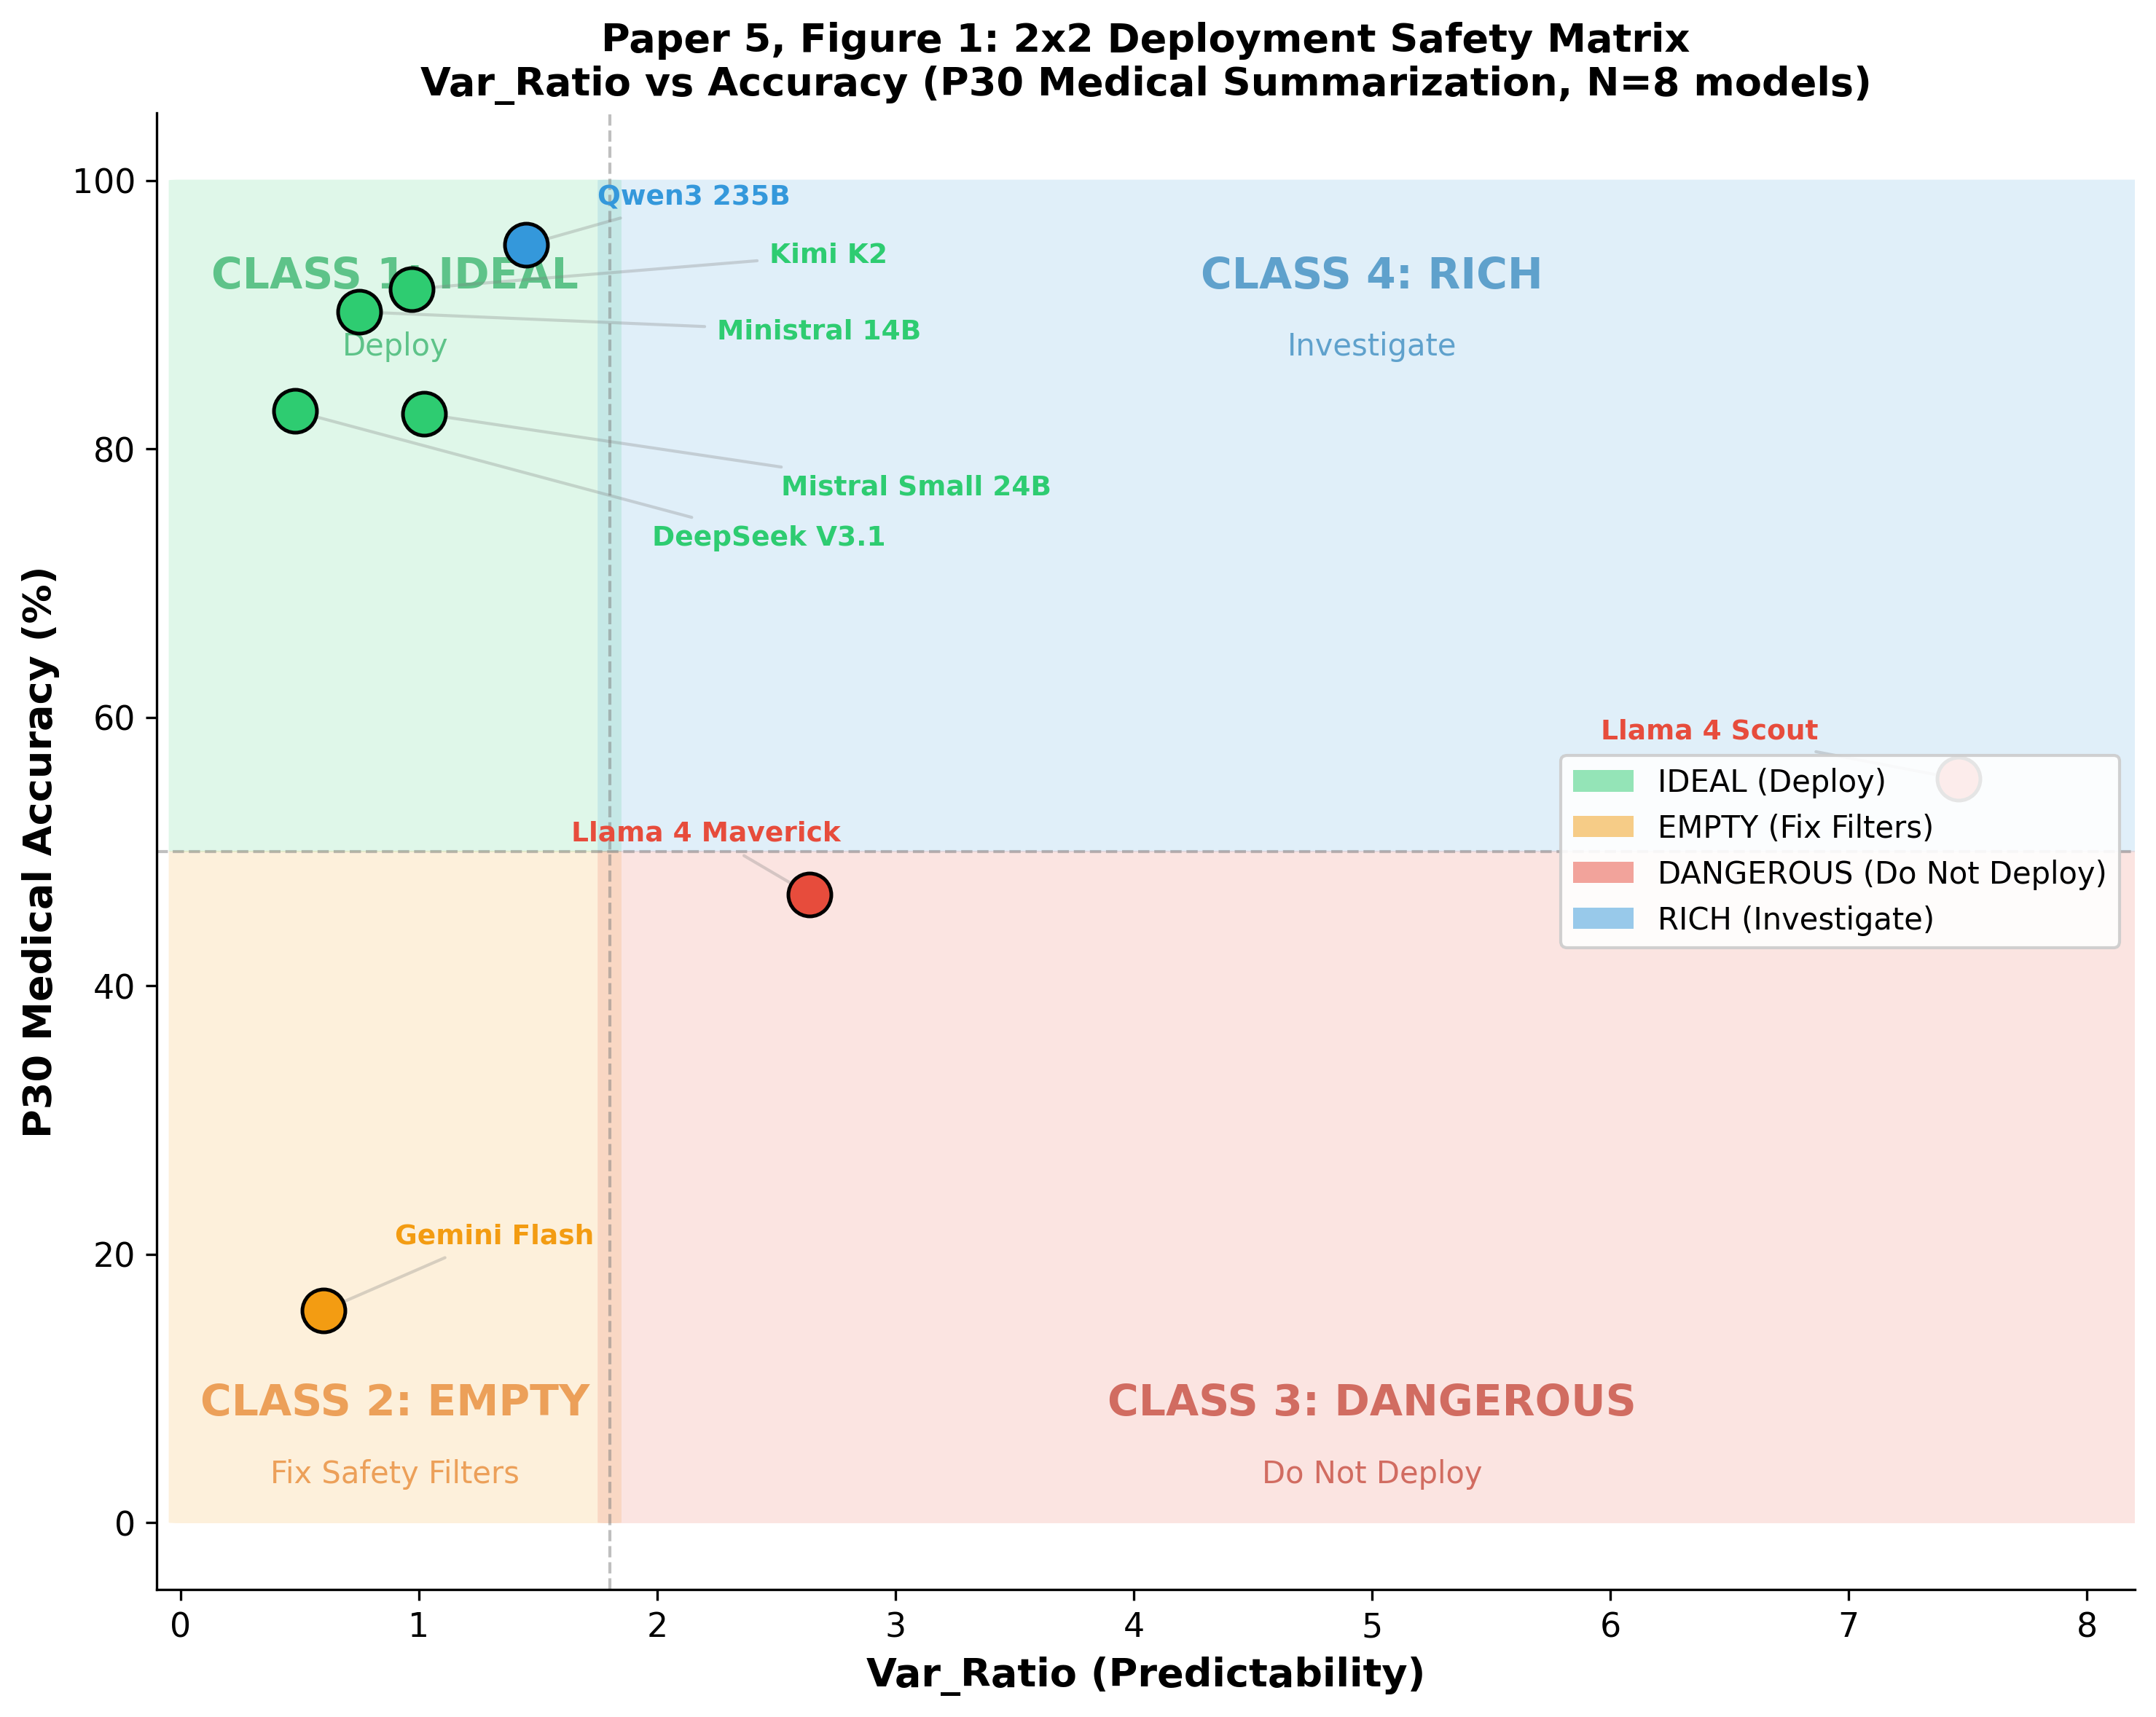
\includegraphics[width=0.80\textwidth]{../figures/fig1_safety_matrix.png}
    \caption{\textbf{The $2 \times 2$ predictability matrix.} Each quadrant represents a distinct behavioral class with different deployment implications. IDEAL: low variance, high accuracy (4 models). EMPTY: low variance, low accuracy (Gemini Flash). DIVERGENT: high variance, moderate accuracy (Llama models). RICH: moderate variance, high accuracy (Qwen3 235B).}
    \label{fig:matrix}
\end{figure}

\textbf{Class 1: IDEAL} (DeepSeek V3.1, Kimi K2, Ministral 14B, Mistral Small 24B). Low $\text{Var\_Ratio}$ ($< 1.2$) with high accuracy (83--92\%). Convergent and comprehensive---outputs are both predictable and clinically complete. These models are suitable for deployment with standard monitoring.

\textbf{Class 2: EMPTY} (Gemini Flash). Low $\text{Var\_Ratio}$ (0.60) with low accuracy (15.8\%). Convergent toward empty or refused responses. The model consistently produces abbreviated outputs that lack clinical detail. This class is invisible to variance-based assessment alone, since low $\text{Var\_Ratio}$ would normally suggest stability.

\textbf{Class 3: DIVERGENT} (Llama 4 Scout, Llama 4 Maverick). High $\text{Var\_Ratio}$ (2.64--7.46) with low-to-moderate accuracy (47--55\%). High trial-to-trial variance correlates with incomplete task coverage. This class exhibits stochastic incompleteness (see Section~\ref{sec:stochastic}).

\textbf{Class 4: RICH} (Qwen3 235B). Moderate $\text{Var\_Ratio}$ (1.45) with high accuracy (95.2\%, 23/50 perfect scores). Diverse surface forms with consistent semantic accuracy. This model produces varied summaries that nonetheless cover clinical elements comprehensively.

\subsection{Stochastic incompleteness: a novel failure mode}
\label{sec:stochastic}

The DIVERGENT class exhibits a failure pattern we term \textbf{stochastic incompleteness}: summaries are factually accurate but randomly incomplete across trials.

\textbf{Element-level analysis} of Llama P30 TRUE-condition responses:

\begin{table}[H]
\centering
\begin{tabular}{lccc}
\toprule
\textbf{Element} & \textbf{Llama Scout} & \textbf{Llama Maverick} & \textbf{DeepSeek V3.1 (IDEAL)} \\
\midrule
STEMI diagnosis & 94\% & 100\% & 100\% \\
PCI performed & 100\% & 100\% & 100\% \\
Age 52 male & 100\% & 100\% & 100\% \\
Chest pain & 96\% & 58\% & 100\% \\
LAD occlusion & 22\% & 6\% & 100\% \\
EF 45\% & 4\% & 2\% & 34\% \\
Cardiac rehab & 16\% & 22\% & 94\% \\
Return to work & 16\% & 0\% & 64\% \\
Follow-up plan & 38\% & 34\% & 54\% \\
\bottomrule
\end{tabular}
\caption{Clinical element hit rates: DIVERGENT vs IDEAL reference. Llama models consistently capture core facts (STEMI, PCI, demographics) but stochastically omit critical details (LAD occlusion, EF, rehabilitation plan).}
\label{tab:elements}
\end{table}

Key observations:

\begin{enumerate}
    \item \textbf{Zero hallucinations} detected across 100 Llama trials (50 Scout + 50 Maverick). All errors are omissions, not fabrications.
    \item \textbf{Core facts are preserved}: STEMI diagnosis, PCI, and patient demographics are consistently present ($>94\%$).
    \item \textbf{Critical details are stochastically omitted}: LAD occlusion, ejection fraction, rehabilitation plan, and follow-up are present in some trials and absent in others. Llama Scout Trial 27 captures 5/16 elements; Trial 11 captures 13/16---same model, same prompt, same context.
    \item \textbf{COLD condition baselines} are near-zero: Scout 1.0/16, Maverick 1.1/16. The models cannot generate clinical summaries without context.
\end{enumerate}

This failure mode is clinically concerning: a physician relying on such a summary would receive an accurate but arbitrarily partial picture, with no indication that information is missing. The output reads as a complete summary---it simply omits different elements each time.

\begin{figure}[H]
    \centering
    
\includegraphics[width=0.85\textwidth]{../figures/fig2_llama_variability.png}
    \caption{\textbf{Trial-level variability in Llama models.} Clinical element coverage varies dramatically across trials under identical conditions. Each bar represents a single trial's element count (out of 16 total). DIVERGENT models show wide dispersion; IDEAL models cluster tightly near maximum coverage.}
    \label{fig:llama}
\end{figure}

\begin{figure}[H]
    \centering
    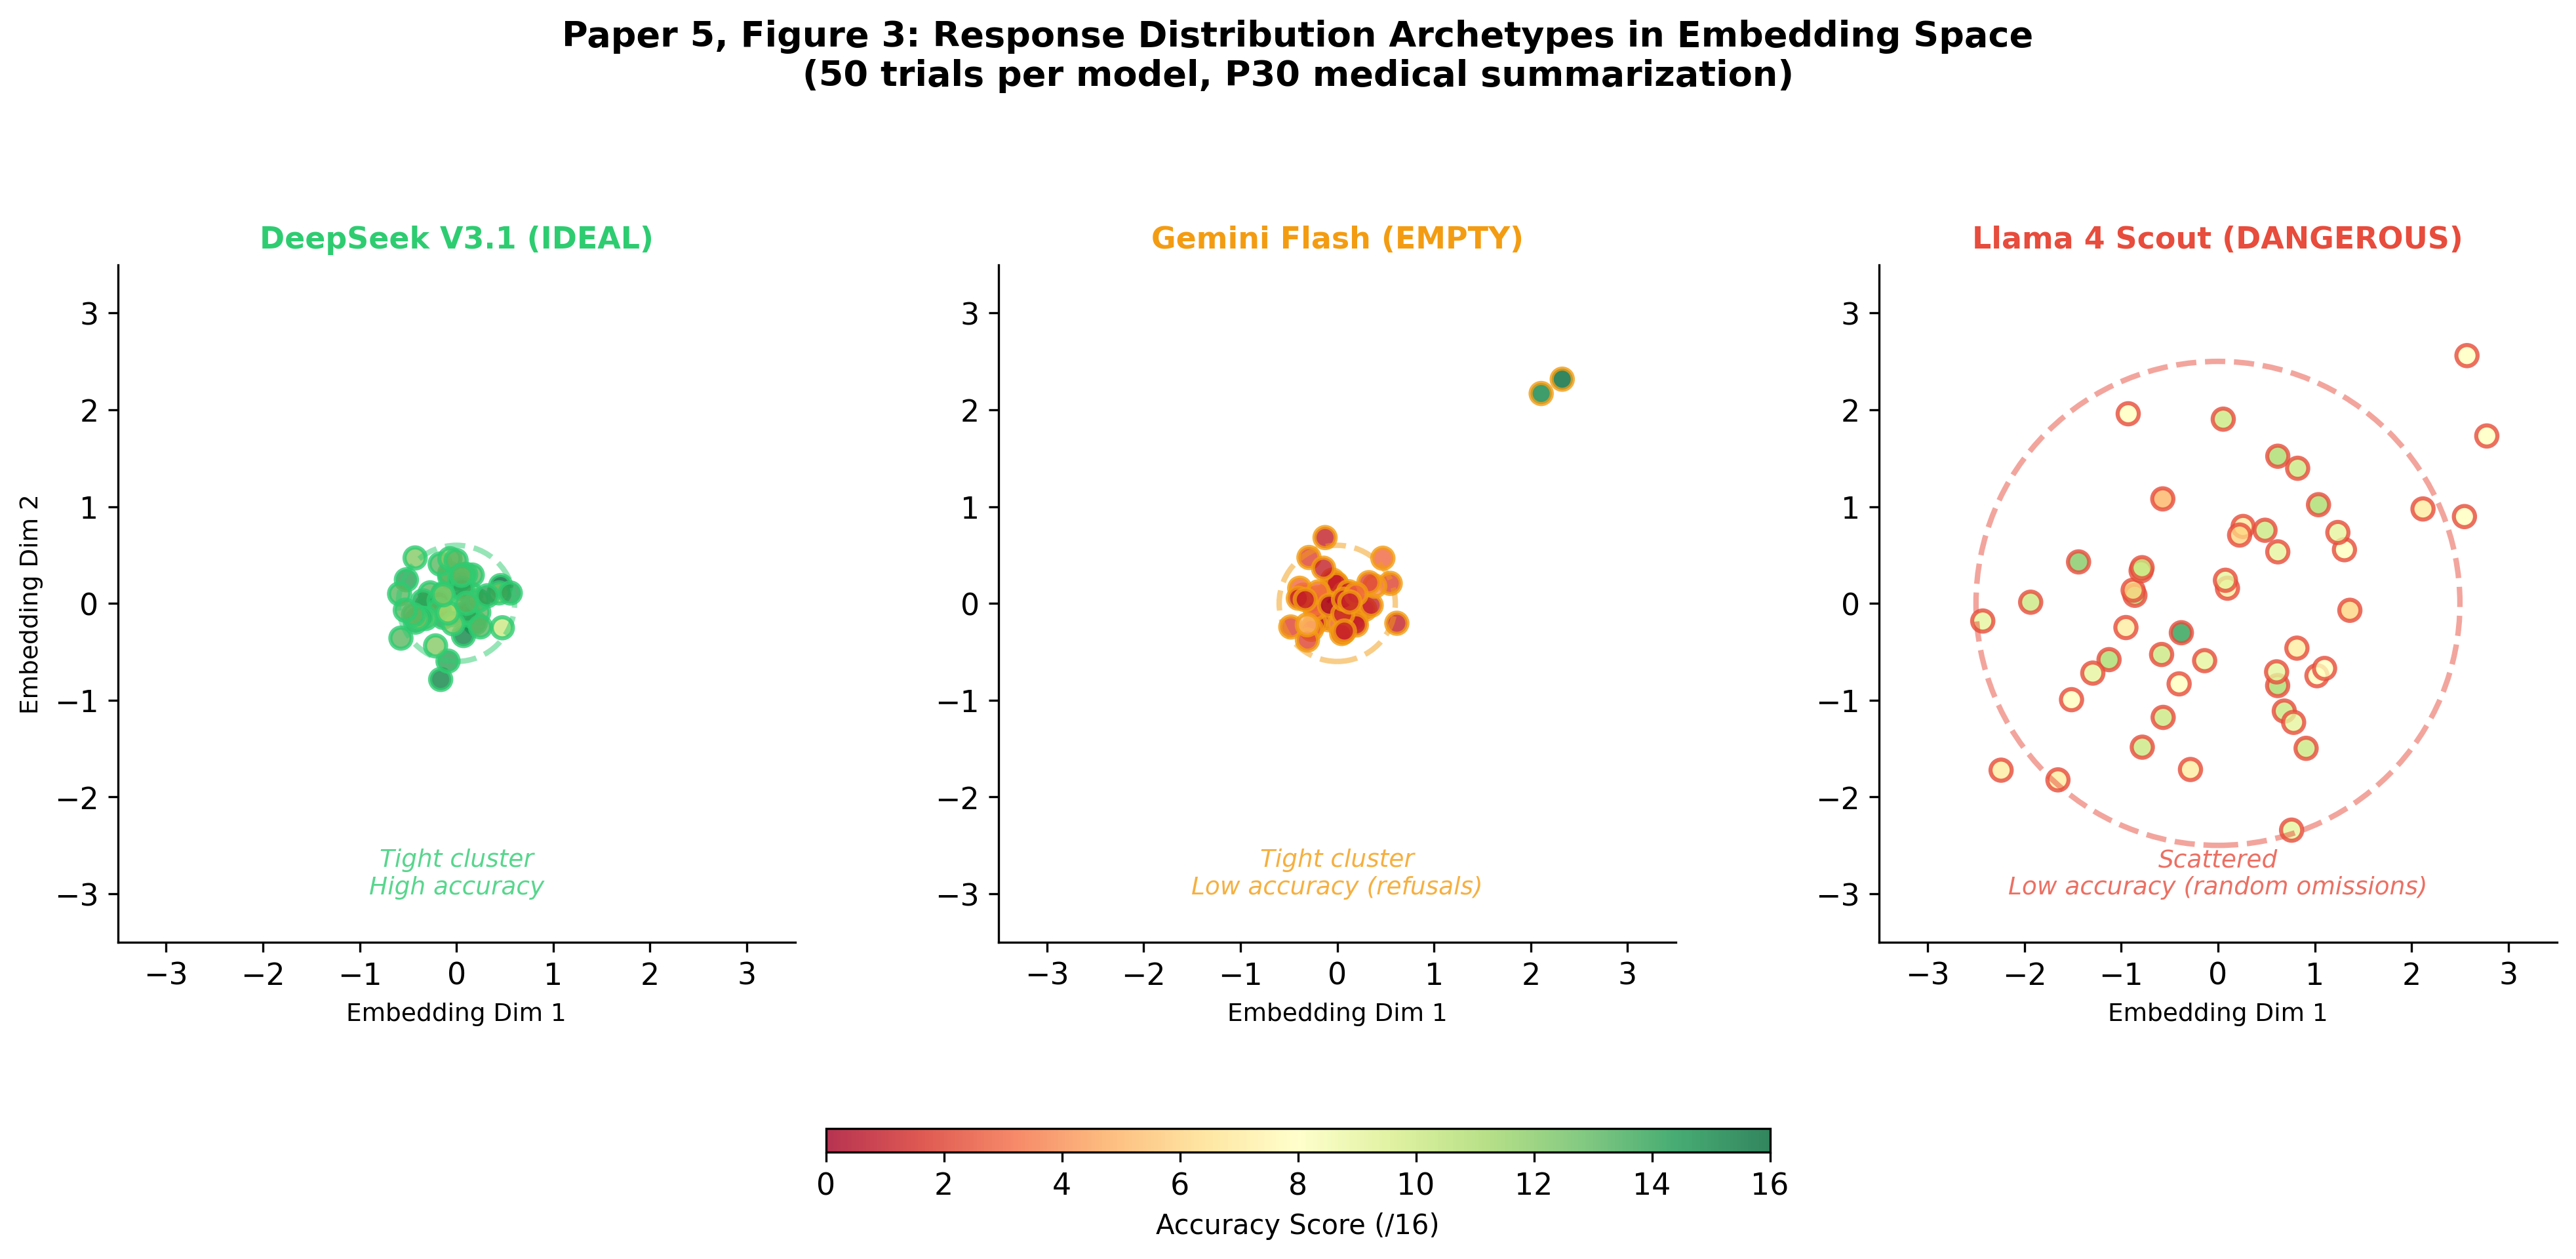
\includegraphics[width=0.85\textwidth]{../figures/fig3_archetypes_embedding.png}
    \caption{\textbf{Response distribution archetypes in embedding space.} IDEAL models cluster tightly; DIVERGENT models show wide dispersion; EMPTY models cluster tightly but in a low-content region. Each point represents one trial's response embedding projected to 2D via PCA.}
    \label{fig:archetypes}
\end{figure}

\subsection{Var\_Ratio thresholds and continuous assessment}

While the four-class taxonomy provides categorical guidance, $\text{Var\_Ratio}$ also supports continuous risk stratification:

\begin{table}[H]
\centering
\begin{tabular}{lcl}
\toprule
\textbf{Var\_Ratio Range} & \textbf{Classification} & \textbf{Interpretation} \\
\midrule
$< 0.8$ & Overly rigid & Risk of empty convergence (EMPTY class) \\
$0.8$--$1.2$ & Stable & Predictable and complete (IDEAL class) \\
$1.2$--$2.0$ & Moderate divergence & Potentially beneficial variation (RICH class) \\
$> 2.0$ & High divergence & Stochastic incompleteness risk (DIVERGENT class) \\
\bottomrule
\end{tabular}
\caption{Empirically motivated $\text{Var\_Ratio}$ thresholds. These boundaries are derived from the current 8-model sample and should be validated on additional models and tasks before adoption as standards.}
\label{tab:thresholds}
\end{table}

\begin{figure}[H]
    \centering
    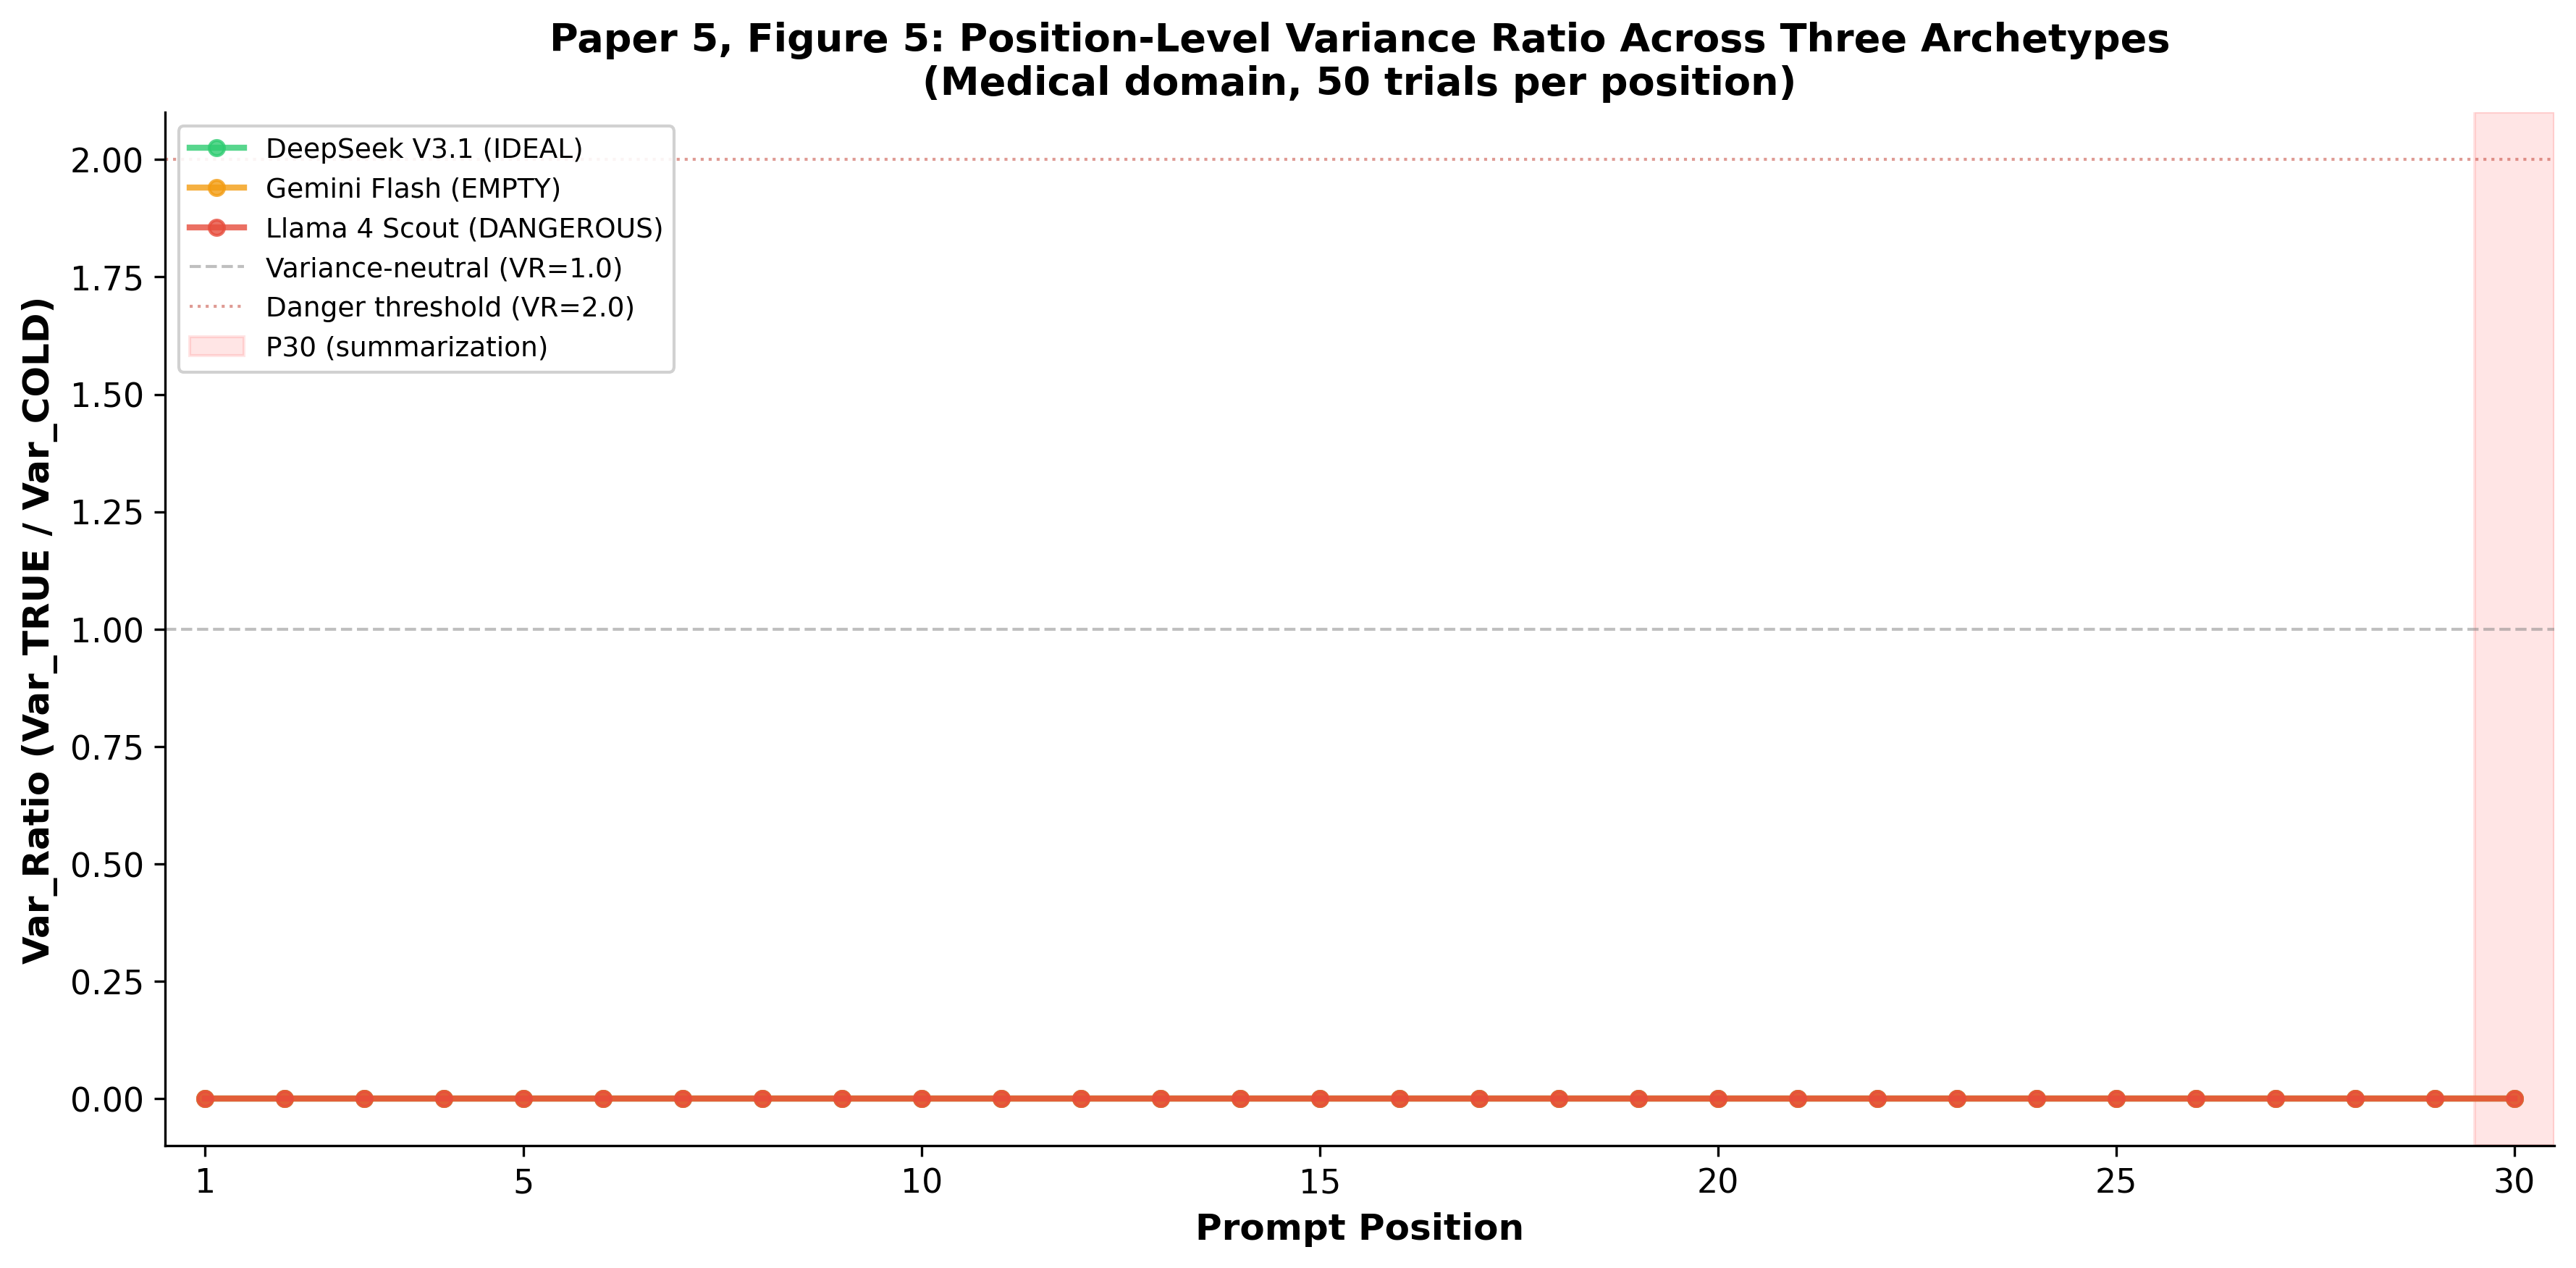
\includegraphics[width=0.85\textwidth]{../figures/fig5_position_var_ratio.png}
    \caption{\textbf{Position-level $\text{Var\_Ratio}$ curves for three archetypal models.} IDEAL models (DeepSeek V3.1) maintain low variance across positions. DIVERGENT models (Llama Scout) show extreme variance spikes at P30. EMPTY models (Gemini Flash) show consistently low variance but poor content coverage.}
    \label{fig:position}
\end{figure}

% ============================================
% 4. DISCUSSION
% ============================================
\section{Discussion}

\subsection{Accuracy is necessary but not sufficient}

The central finding is that accuracy and output predictability are independent dimensions. A model with acceptable aggregate accuracy (Llama Scout, 55\%) can produce individual summaries that range from clinically adequate (13/16 elements) to dangerously incomplete (5/16 elements). Conversely, a model with highly predictable outputs (Gemini Flash, $\text{Var\_Ratio} = 0.60$) can be consistently wrong (15.8\% accuracy). Neither dimension alone captures the full deployment risk.

\subsection{Stochastic incompleteness as a failure mode}

Standard hallucination detection focuses on fabricated content \citep{asgari2025framework}. Stochastic incompleteness is a complementary failure mode: content is accurate but arbitrarily partial. This is arguably more dangerous than hallucination in clinical settings, because omissions are harder to detect than fabrications. A hallucinated lab value can be flagged as inconsistent; a missing follow-up plan simply does not appear in the summary.

The term ``stochastic incompleteness'' captures the core mechanism: each trial samples a different subset of the available clinical information, with no systematic pattern to the omissions. The result is a model that is correct but unreliable---factually sound on any given element it includes, but unpredictable in which elements it includes.

\subsection{The RICH class: beneficial divergence}

Qwen3 235B achieves the highest accuracy (95.2\%) with moderate variance ($\text{Var\_Ratio} = 1.45$). This suggests that some output diversity may be compatible with---or even beneficial for---task completeness, provided the model consistently covers the required elements despite surface-level variation. The RICH class is small ($N = 1$) and should be studied further, but it provides a counterexample to the assumption that lower variance is always better.

\subsection{Deployment framework}

We propose a minimum two-dimensional assessment for clinical AI deployment:

\begin{enumerate}
    \item \textbf{Accuracy assessment}: Score against a task-specific rubric across multiple trials.
    \item \textbf{Predictability assessment}: Compute $\text{Var\_Ratio}$ across those same trials.
    \item \textbf{Classify}: Map into the four-class taxonomy.
    \item \textbf{Decide}: IDEAL $\to$ deploy with monitoring; EMPTY $\to$ reconfigure; DIVERGENT $\to$ do not deploy in current form; RICH $\to$ investigate further.
\end{enumerate}

\begin{figure}[H]
    \centering
    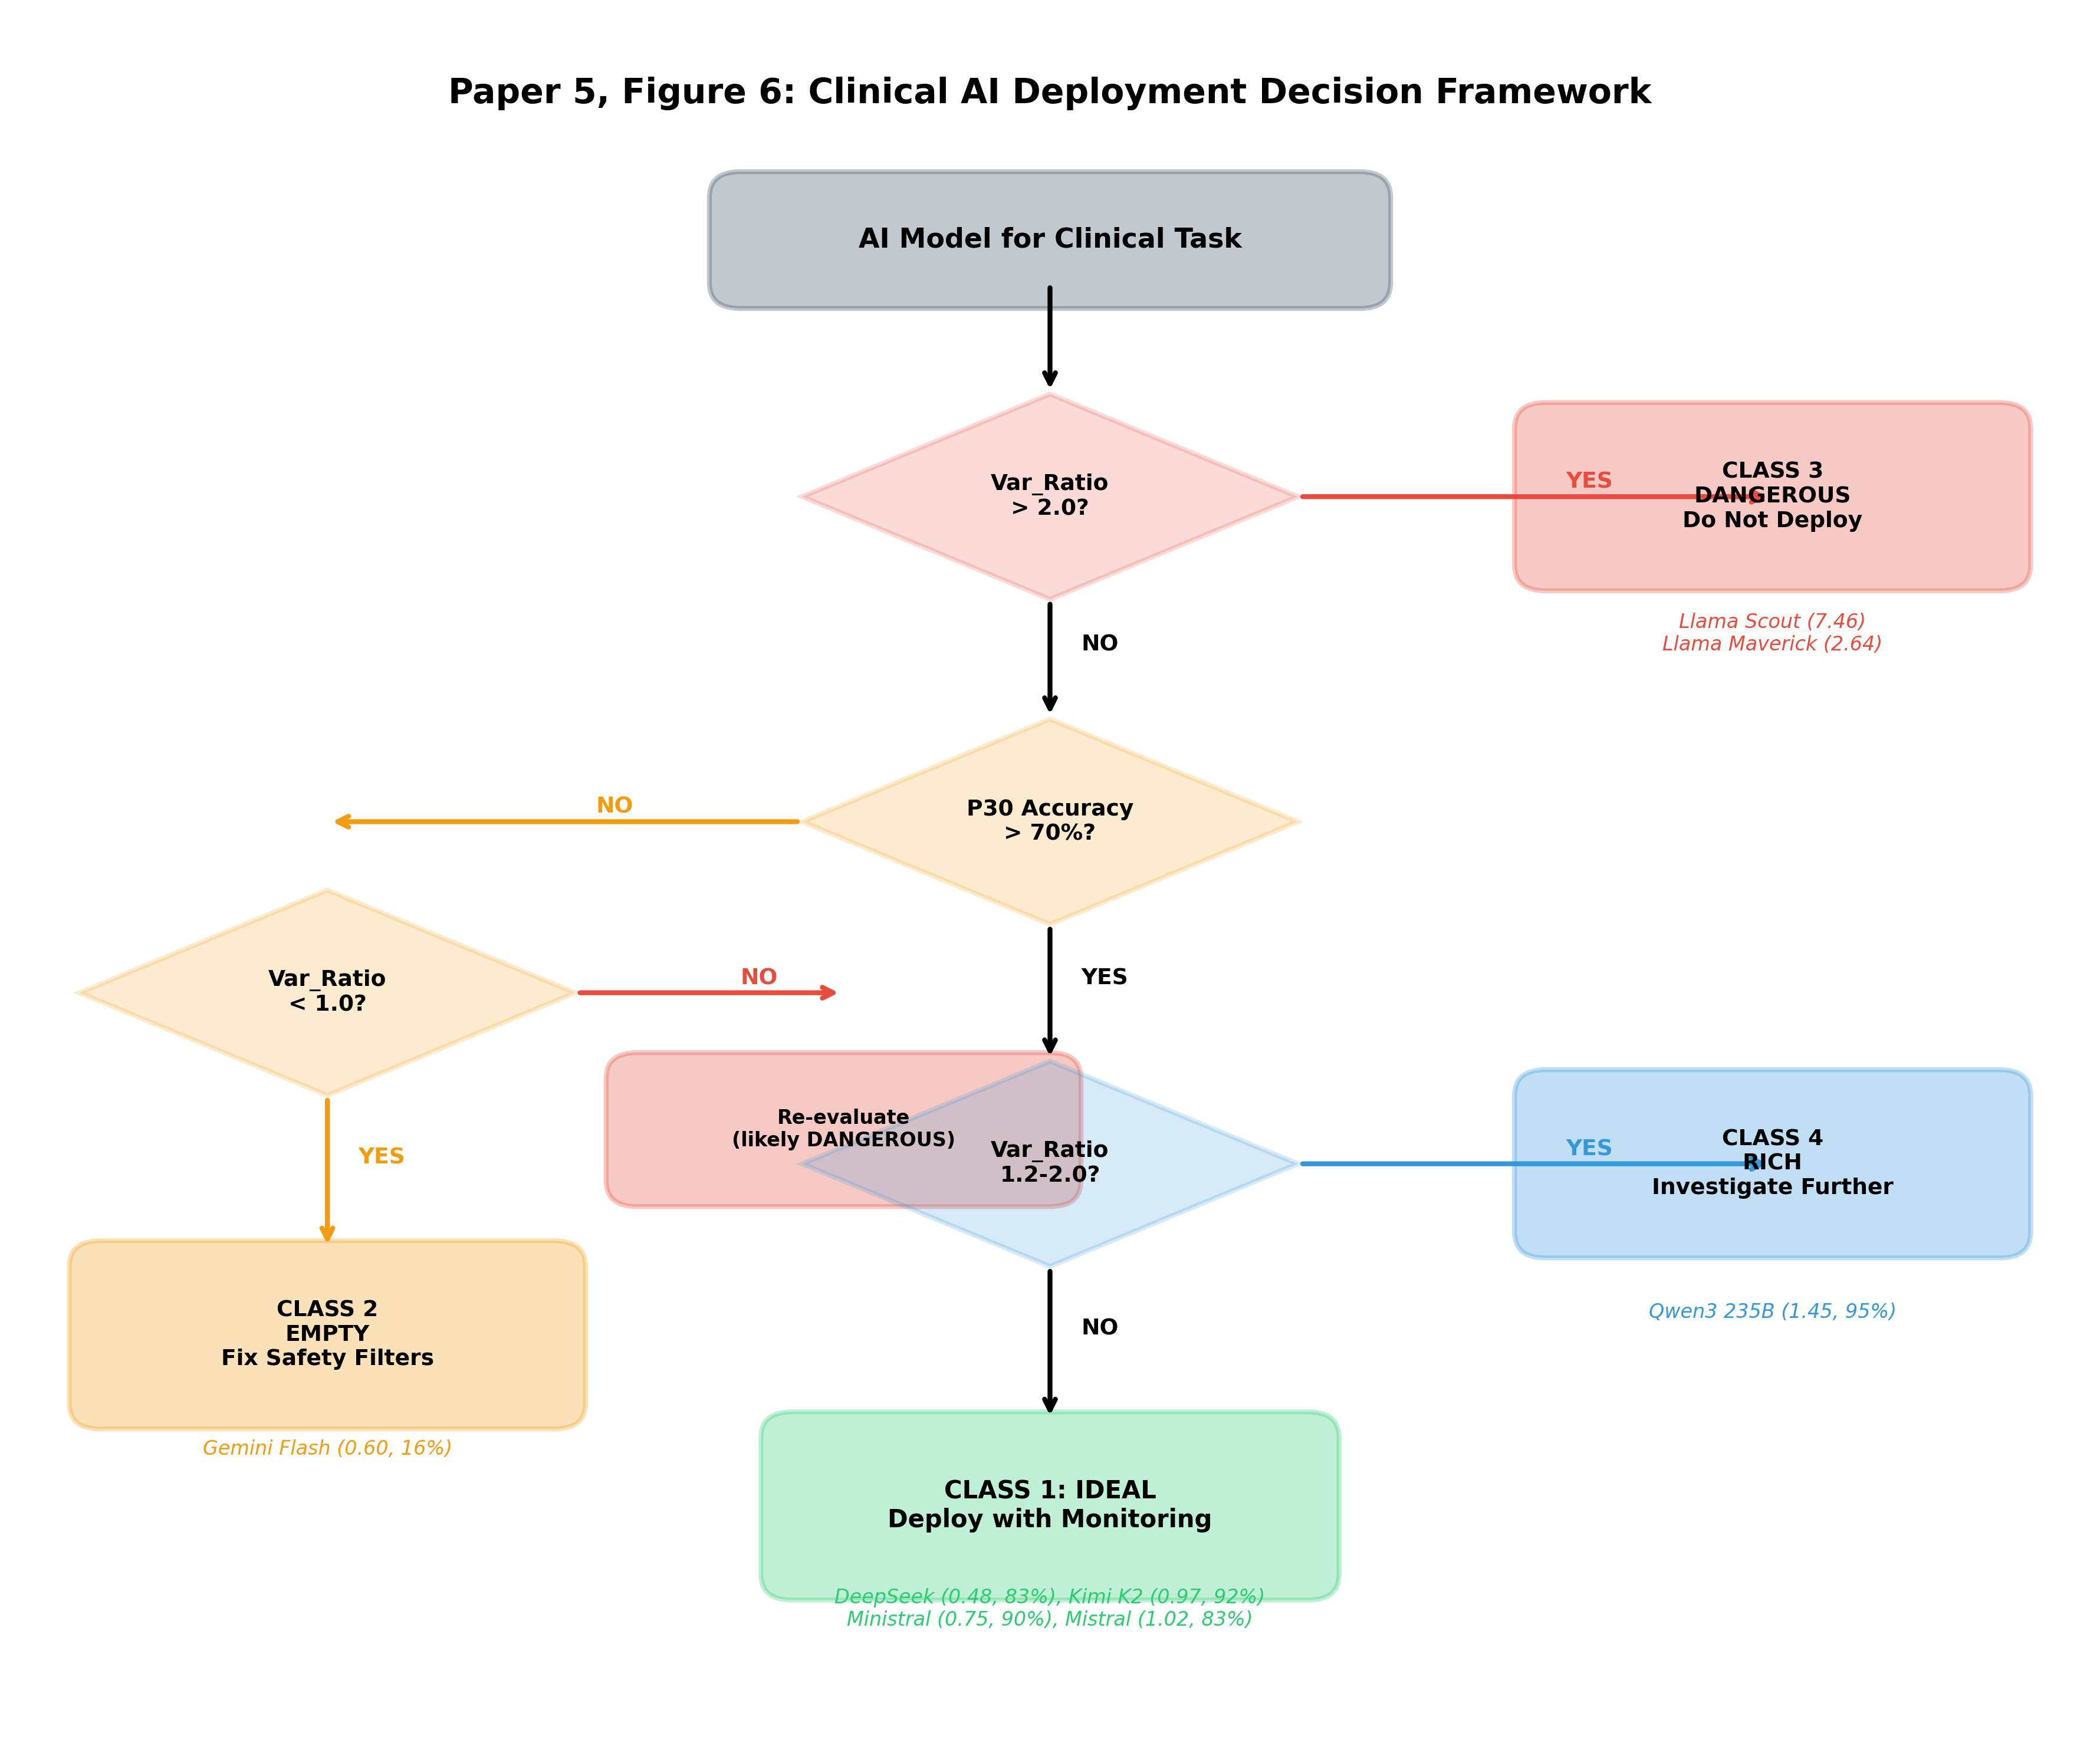
\includegraphics[width=0.85\textwidth]{../figures/fig6_deployment_flowchart.png}
    \caption{\textbf{Deployment decision framework.} Both accuracy and $\text{Var\_Ratio}$ are required; neither alone is sufficient. The flowchart guides deployment decisions based on combined assessment.}
    \label{fig:deployment}
\end{figure}

\subsection{Future Directions}

Several research directions emerge from this taxonomy. First, \textbf{Context Utilization Depth (CUD)} experiments currently in preparation will test whether models with high predictability (IDEAL class) can effectively integrate longer context windows, or whether engagement depth trades off against stability. Preliminary pilot data from 4 models (DeepSeek V3.1, Gemini Flash, Llama 4 Maverick, Qwen3 235B) suggest that Medical domain requires deeper context integration ($K > 15$ messages) than Philosophy domain ($K < 5$ messages), consistent with the task-specific predictability signatures observed here.

Second, the taxonomy should be validated across additional clinical tasks (radiology reports, discharge summaries, differential diagnosis) to determine whether the four classes represent generalizable behavioral archetypes or position-specific patterns. If the IDEAL/EMPTY/DIVERGENT/RICH distinction holds across diverse clinical scenarios, it would suggest fundamental differences in how models handle task-critical summarization under context.

Third, longitudinal studies tracking $\text{Var\_Ratio}$ and accuracy across model versions could reveal whether architectural improvements enhance both dimensions simultaneously or redistribute existing capacity between predictability and completeness. The observation that Qwen3 235B achieves both high accuracy and moderate variance (RICH class) while other large models show trade-offs suggests that scale alone is not sufficient---training objectives and safety tuning may play critical roles.

Finally, the relationship between stochastic incompleteness and the ``Lost in Conversation'' phenomenon documented by Laban et al.\ \citeyearpar{laban2025lost} warrants investigation. Models that exhibit divergent entanglement (Paper~4) at task-critical positions may be prone to stochastic incompleteness under multi-turn settings, providing a mechanistic link between variance signatures and clinical deployment risk.

\subsection{Limitations}

\textbf{Sample size.} Eight models in a single domain (medical P30). The taxonomy may not generalize to other tasks or positions.

\textbf{Accuracy rubric.} The 16-element rubric is specific to the STEMI case. Different clinical scenarios would require different rubrics, and the element granularity affects accuracy scores.

\textbf{Var\_Ratio computation.} P30-specific $\text{Var\_Ratio}$ values differ from model-level averages. The taxonomy is valid at P30 but may not apply at other positions.

\textbf{Class boundaries.} The IDEAL/RICH boundary ($\text{Var\_Ratio} = 1.2$) and DIVERGENT threshold ($\text{Var\_Ratio} > 2.0$) are empirically motivated from 8 models. Larger samples may refine these boundaries.

\textbf{Single embedding model.} $\text{Var\_Ratio}$ depends on the all-MiniLM-L6-v2 embedding space. Alternative embedding models may yield different variance distributions.

% ============================================
% 5. CONCLUSION
% ============================================
\section{Conclusion}

We demonstrate that accuracy and output predictability are independent dimensions for clinical AI assessment ($r = -0.24$, $p = 0.56$). This independence yields a four-class behavioral taxonomy---IDEAL, EMPTY, DIVERGENT, RICH---that captures failure modes invisible to either dimension alone.

The DIVERGENT class exhibits stochastic incompleteness: summaries that are factually sound but randomly incomplete, with zero hallucinations and no warning of missing information. This failure mode is undetectable by standard accuracy benchmarks, which report adequate mean performance while masking extreme trial-to-trial variability.

The EMPTY class demonstrates a complementary blind spot: convergent outputs that standard variance metrics would classify as stable but that lack clinical content entirely.

We propose that any deployment assessment for clinical AI should evaluate both accuracy (via task-specific rubrics) and predictability (via $\text{Var\_Ratio}$ or equivalent) across multiple independent trials. Single-trial evaluation is insufficient for safety-critical applications.

% ============================================
% ACKNOWLEDGMENTS
% ============================================
\section*{Acknowledgments}

This research builds on the MCH Research Program established in Papers~1--4. AI systems (Claude, ChatGPT, DeepSeek) assisted with data analysis, visualization, and manuscript preparation. The framework, findings, and interpretations remain the author's sole responsibility.

% ============================================
% DATA AVAILABILITY
% ============================================
\section*{Data Availability}

All raw data, response text, and analysis scripts are available in the project repository:

\noindent\url{https://github.com/LaxmanNandi/MCH-Research}

\noindent Specific data locations:
\begin{itemize}
    \item Cross-model accuracy results: \texttt{data/paper5/accuracy\_verification/}
    \item Llama trial-level analysis: \texttt{data/paper5/llama\_deep\_dive/}
    \item Model response data: \texttt{data/medical/} (shared with Paper~2)
\end{itemize}

% ============================================
% REFERENCES
% ============================================
\bibliographystyle{plainnat}
\begin{thebibliography}{20}

\bibitem[Laban et al., 2025]{laban2025lost}
Laban, P., Hayashi, H., Zhou, Y., \& Neville, J.\ (2025).
\newblock LLMs get lost in multi-turn conversation.
\newblock {\em arXiv preprint}, arXiv:2505.06120.

\bibitem[Laxman, 2026a]{laxman2026paper1}
Laxman, M.\ M.\ (2026a).
\newblock Context curves behavior: Measuring AI relational dynamics with $\Delta$RCI.
\newblock {\em Preprints.org}, 202601.1881. DOI:~10.20944/preprints202601.1881.v2

\bibitem[Laxman, 2026b]{laxman2026paper2}
Laxman, M.\ M.\ (2026b).
\newblock Scaling context sensitivity: A standardized benchmark of $\Delta$RCI across 25 model-domain runs.
\newblock {\em Preprints.org}, 202602.1114. DOI:~10.20944/preprints202602.1114.v2

\bibitem[Laxman, 2026c]{laxman2026paper3}
Laxman, M.\ M.\ (2026c).
\newblock Domain-specific temporal dynamics of context sensitivity in large language models.
\newblock {\em Preprints.org}, ID:~199272.

\bibitem[Laxman, 2026d]{laxman2026paper4}
Laxman, M.\ M.\ (2026d).
\newblock Engagement as entanglement: Variance signatures of bidirectional context coupling in large language models.
\newblock In preparation.

\bibitem[Laxman, 2026e]{laxman2026paper6}
Laxman, M.\ M.\ (2026e).
\newblock An empirical conservation constraint on context sensitivity and output variance:
Evidence across LLM architectures.
\newblock In preparation.

\bibitem[Asgari et al., 2025]{asgari2025framework}
Asgari, E., et al.\ (2025).
\newblock A framework to assess clinical safety and hallucination rates of LLMs
for medical text summarisation.
\newblock {\em npj Digital Medicine}, 8(1), 274.

\bibitem[Reimers \& Gurevych, 2019]{reimers2019sentence}
Reimers, N., \& Gurevych, I.\ (2019).
\newblock Sentence-BERT: Sentence embeddings using Siamese BERT-networks.
\newblock {\em Proceedings of EMNLP 2019}.

\bibitem[Brown et al., 2020]{brown2020language}
Brown, T., Mann, B., Ryder, N., Subbiah, M., et al.\ (2020).
\newblock Language models are few-shot learners.
\newblock {\em Advances in Neural Information Processing Systems}, 33.

\bibitem[Vaswani et al., 2017]{vaswani2017attention}
Vaswani, A., Shazeer, N., Parmar, N., Uszkoreit, J., Jones, L., Gomez, A.\ N.,
Kaiser, \L., \& Polosukhin, I.\ (2017).
\newblock Attention is all you need.
\newblock {\em Advances in Neural Information Processing Systems}, 30.

\bibitem[Liu et al., 2024]{liu2024lost}
Liu, N.\ F., Lin, K., Hewitt, J., Paranjape, A., Bevilacqua, M., Petroni, F.,
\& Liang, P.\ (2024).
\newblock Lost in the middle: How language models use long contexts.
\newblock {\em Transactions of the Association for Computational Linguistics}, 12, 104--123.

\bibitem[Rajkomar et al., 2018]{rajkomar2018scalable}
Rajkomar, A., Oren, E., Chen, K., Dai, A.\ M., Hajaj, N., Hardt, M., et al.\ (2018).
\newblock Scalable and accurate deep learning with electronic health records.
\newblock {\em npj Digital Medicine}, 1(1), 18.

\bibitem[Singhal et al., 2023]{singhal2023med}
Singhal, K., Azizi, S., Tu, T., Mahdavi, S.\ S., Wei, J., Chung, H.\ W., et al.\ (2023).
\newblock Large language models encode clinical knowledge.
\newblock {\em Nature}, 620(7972), 172--180.

\bibitem[Thirunavukarasu et al., 2023]{thirunavukarasu2023large}
Thirunavukarasu, A.\ J., Ting, D.\ S.\ J., Elangovan, K., Gutierrez, L., Tan, T.\ F., \& Ting, D.\ S.\ W.\ (2023).
\newblock Large language models in medicine.
\newblock {\em Nature Medicine}, 29(8), 1930--1940.

\end{thebibliography}

\end{document}
